\documentclass{standalone}
\usepackage{tikz}
\usepackage[colorlinks=true]{hyperref}
\usetikzlibrary{
  arrows,
  calc,
  decorations.pathmorphing,
  decorations.pathreplacing,
  decorations.markings,
  fadings,
  positioning,
  shapes,
  arrows.meta
}
\tikzfading[name = lens fading,inner color = transparent!0,outer color = transparent!100]
\tikzfading[name = pbs fading,top color = transparent!0,bottom color = transparent!100]
\tikzset{
  mid arrow/.style={postaction={decorate,decoration={
        markings,
        mark=at position .5 with {\arrow[#1]{stealth}}
      }}},
  mid arrow2/.style={postaction={decorate,decoration={
        markings,
        mark=at position .5 with {\arrow[>=stealth]{><}}
      }}},
}

\newcommand\drawellipseshade[5][inner color=black,outer color=black]{
  % 1: shading option
  % 2: center (x, y)
  % 3: xsize
  % 4: ysize
  % 5: angle
  \begin{scope}
    \clip[rotate around={#5:#2}] #2 ellipse ({#3} and {#4});
    \begin{scope}[transform canvas={shift={#2}, rotate=#5}]
      \shade[shading=radial,path fading=lens fading, #1] (0, 0) ellipse ({#3} and {#4});
    \end{scope}
  \end{scope}
}
% \newcommand\drawlens[3]{
%   % 1: center (x, y)
%   % 2: size
%   % 3: angle
%   \drawellipseshade[inner color=blue,outer color=blue!40!cyan]{#1}{#2}{{0.14 * #2}}{#3}
% }
% \newcommand\drawwaveplate[3]{
%   % 1: center (x, y)
%   % 2: size
%   % 3: angle
%   \drawellipseshade[inner color=blue!50!black,outer color=blue!80!black]{#1}{#2}{{0.07 * #2}}{#3}
% }
% \newcommand\drawaom[4]{
%   % 1: center (x, y)
%   % 2: xsize
%   % 3: ysize
%   % 4: angle
%   \drawellipseshade[inner color=orange,outer color=orange]{#1}{#2}{#3}{#4}
%   \begin{scope}[rotate around={#4:#1}]
%     \fill[orange, even odd rule, opacity=0.8]
%     ($#1 + ({#2}, 0)$) arc (0:360:{#2} and {#3})
%     -- ($#1 + ({#2}, {#3})$) -- ($#1 + (-{#2}, {#3})$) -- ($#1 + (-{#2}, -{#3})$)
%     -- ($#1 + ({#2}, -{#3})$) --cycle;
%     \draw ($#1 + ({#2}, {#3})$) -- ($#1 + (-{#2}, {#3})$) -- ($#1 + (-{#2}, -{#3})$)
%     -- ($#1 + ({#2}, -{#3})$) --cycle;
%   \end{scope}
% }
% \newcommand\drawpbs[3]{
%   % 1: center (x, y)
%   % 2: size
%   % 3: angle
%   \begin{scope}
%     \begin{scope}
%       \clip[rotate around={#3:#1}] ($#1 - ({#2}, {#2})$) rectangle ($#1 + ({#2}, {#2})$);
%       \begin{scope}[transform canvas={shift={#1}, rotate=#3}]
%         \shade[bottom color=blue!60!cyan, top color=blue!50!cyan, path fading=pbs fading]
%         (-{#2}, -{#2}) rectangle ({#2}, {#2});
%         \draw[line width=1] (-{#2}, -{#2}) -- ({#2}, {#2});
%       \end{scope}
%     \end{scope}
%     % Make sure the frame is not clipped
%     \draw[rotate around={#3:#1}] ($#1 - ({#2}, {#2})$) rectangle ($#1 + ({#2}, {#2})$);
%   \end{scope}
% }
\newcommand\drawlens[3]{
  % 1: center (x, y)
  % 2: size
  % 3: angle
  \begin{scope}[shift={#1}]
    \node[rotate={#3}] at (0, 0) {\scalebox{#2}{
\includegraphics[width=2cm]{lens.png}}};
  \end{scope}
}
\newcommand\drawwaveplate[3]{
  % 1: center (x, y)
  % 2: size
  % 3: angle
  \begin{scope}[shift={#1}]
    \node[rotate={#3}] at (0, 0) {\scalebox{#2}{
\includegraphics[width=2cm]{wp.png}}};
  \end{scope}
}
\newcommand\drawaom[4]{
  % 1: center (x, y)
  % 2: xsize
  % 3: ysize
  % 4: angle
  \begin{scope}[shift={#1}]
    \node[rotate={#4}] at (0, 0)
    {\scalebox{#2}[#3]{
\includegraphics[width=2cm,height=2cm]{AOM.png}}};
  \end{scope}
}
\newcommand\drawpbs[3]{
  % 1: center (x, y)
  % 2: size
  % 3: angle
  \begin{scope}[shift={#1}]
    \node[rotate={#3}] at (0, 0)
    {\scalebox{#2}{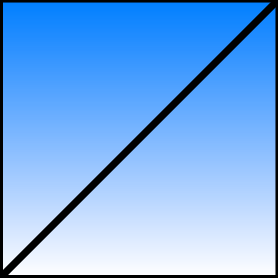
\includegraphics[width=1.4285714285714286cm]{PBS.png}}};
  \end{scope}
}

\ifpdf
% Ensure reproducible output
\pdfinfoomitdate=1
\pdfsuppressptexinfo=-1
\pdftrailerid{}
\hypersetup{
  pdfcreator={},
  pdfproducer={}
}
\fi

\begin{document}

\begin{tikzpicture}
  % Input
  \node[red,above] at (2, 0) {\large\textbf{From Laser}};
  \draw[red,line width=1.6,mid arrow] (2, 0) -- (0, 0);
  % Wavemeter
  \draw[red,line width=1.6] (0, 0) -- (0, -1);
  \draw[red,line width=1.6,mid arrow] (0, -1) -- (0, -2);
  \node[red,below] at (0, -2) {\large\textbf{To wavemeter}};
  % Between PBS and DP AOM
  \draw[red,line width=1.6,mid arrow2] (-2, 0) -- (0, 0);
  \begin{scope}
    % Clip off one arrow
    \clip (-1.23, 0) rectangle (-2, 1);
    \draw[blue,line width=1.6,mid arrow2] (-2, 0) -- (0, 0);
  \end{scope}
  \begin{scope}
    % Redraw the clipped line
    \clip (0, 0) rectangle (-2, 1);
    \draw[blue,line width=1.6] (-2, 0) -- (0, 0);
  \end{scope}
  % Output
  \draw[red,line width=1.6] (0, 0) -- (0, 1);
  \draw[red,line width=1.6,mid arrow] (0, 1) -- (0, 2);
  \begin{scope}
    \clip (0, 0) rectangle (-1, 3);
    \draw[blue,line width=1.6] (0, 0) -- (0, 1);
    \draw[blue,line width=1.6,mid arrow] (0, 1) -- (0, 2);
  \end{scope}
  \node[red] at (0, 2.3) {\large\textbf{To Experiment}};
  \begin{scope}
    \clip (-2, 2.3) rectangle (2, 3.5);
    \node[blue] at (0, 2.3) {\large\textbf{To Experiment}};
  \end{scope}
  \draw[red,line width=1.6,mid arrow2] (-2, 0) -- (-6, 0);
  \draw[blue,line width=1.6,mid arrow2] (-2, 0) --
  node[above,pos=0.34,rotate=-5] {\small $\approx\!+345~\mathrm{MHz}$} (-6 - 0.3, 0 + 0.3);
  \draw[blue,line width=1.6,mid arrow2] (-6 - 0.3, 0 + 0.3) -- (-6 - 0.4, 2.5 + 0.05);
  \draw[red,line width=1.6,mid arrow2] (-6, 0) -- (-6, 5);
  \draw[red,line width=1.6,mid arrow2] (-7.5, 5) -- (-6, 5);
  \draw[red,line width=1.6] (-7.5, 5) -- (-9, 5);
  \draw[red,line width=1.6] (-9, 5) -- (-10, 5);
  \draw[red,line width=1.6,mid arrow] (-10, 5) -- (-11.5, 5);
  \draw[red,line width=1.6] (-11.5, 5) -- (-11.5, 3.3);
  \draw[red,line width=1.6,mid arrow] (-11.5, 3.3) --
  node[above,rotate=86,pos=0.45] {\small $-80~\mathrm{MHz}$} (-11.5 - 0.2, 0 + 0.2);
  \draw[red,line width=1.6,mid arrow] (-11.5 - 0.2, 0 + 0.2) -- (-9, 0);
  \draw[red,line width=1.6,mid arrow] (-9, 0) -- (-9, 5);
  % Input PBS
  \drawpbs{(0, 0)}{0.7}{0}
  \node[blue!40!cyan,below right] at (0 + 0.7, 0 - 0.7) {\large PBS 1};
  % DP AOM
  \drawaom{(-2, 0)}{1}{0.5}{90}
  \node[rotate=-90] at (-2, 0) {\large DP AOM};
  % DP Lens
  % \node[rotate=90] at (-4.5, 0) {
\includegraphics[width={2 cm}]{lens.pdf}};
  \drawlens{(-4.5, 0)}{1}{90}
  \node[blue!80!cyan,below] at (-4.5, -1) {\large L1};
  \draw[line width=3] (-6 - 0.7, 0 + 0.7) -- (-6 + 0.7, 0 - 0.7);
  % DP QWP
  \drawwaveplate{(-6, 1.5)}{1}{0}
  \node[blue!80!black,right] at (-5.1, 1.5) {\large $\lambda/4$};
  \draw[line width=3,shift={(-6 - 0.4, 2.5 + 0.05)}] (-0.3, -0.02) -- (0.3, 0.02);
  % Post DP QWP
  \drawwaveplate{(-6, 3.5)}{1}{0}
  \node[blue!80!black,right] at (-5.1, 3.5) {\large $\lambda/4$};
  \draw[line width=3] (-6 - 0.7, 5 + 0.7) -- (-6 + 0.7, 5 - 0.7);
  % Post DP Lens
  \drawlens{(-7.5, 5)}{1}{90}
  \node[blue!80!cyan,above] at (-7.5, 6) {\large L2};
  % SP PBS
  \drawpbs{(-9, 5)}{0.7}{0}
  \node[blue!40!cyan,above] at (-9, 5 + 0.7) {\large PBS 2};
  \draw[line width=3] (-11.5 - 0.7, 5 - 0.7) -- (-11.5 + 0.7, 5 + 0.7);
  % SP AOM
  \drawaom{(-11.5, 3.3)}{1}{0.5}{0}
  \node at (-11.5, 3.3) {\large SP AOM};
  \draw[line width=3] (-11.5 - 0.7, 0 + 0.7) -- (-11.5 + 0.7, 0 - 0.7);
  \draw[line width=3] (-9 - 0.7, 0 - 0.7) -- (-9 + 0.7, 0 + 0.7);
  % SP HWP
  \drawwaveplate{(-9, 1.7)}{1}{0}
  \node[blue!80!black,left] at (-9.9, 1.7) {\large $\lambda/2$};

  \draw[gray,opacity=0.8,line width=1,dashed] (-4, 6) |- (2.8, 2.8);

  \begin{scope}[shift={(-1.4, 4)}]
    \draw[red,line width=1.6,mid arrow] (3, 0) node[below] {\large\textbf{Input}} -- (0, 0);
    \draw[red,line width=1.6,mid arrow] (0, 0) -- ({3 * cos(40)}, {3 * sin(40)})
    node[left] {\large\textbf{Output}};
    \draw[gray,line width=6] ({-0.7 * tan(20)}, 0.7) --
    node[black,left] {\large ASE Filter} ({0.7 * tan(20)}, -0.7);
  \end{scope}
\end{tikzpicture}

\end{document}
